\chapter{Los multipletes de \texorpdfstring{\(SU(5)\)}{SU(5)}, los bosones gauge leptoquarks y la desintegración del protón}

\lectureoverview{La gran unificación se vuelve concreta cuando el grupo del Modelo Estándar se incorpora en \(SU(5)\). Para entender qué significa esta afirmación, primero desarrollamos la teoría de representaciones necesaria: la representación definitoria \(N\), su conjugada \(\overline N\), los productos tensoriales, los tensores simétricos y antisimétricos, y la representación adjunta. Una familia del Modelo Estándar queda entonces reunida en la combinación, inesperadamente económica, \(\overline{\mathbf 5}\oplus\mathbf{10}\). La misma simetría que hace bella esta organización también exige bosones gauge coloreados que convierten quarks en leptones. Su intercambio permite la desintegración del protón y obliga a situar la escala de unificación cerca de \(10^{15}\)--\(10^{16}\,\mathrm{GeV}\). Los acoplamientos gauge que evolucionan con la escala apuntan a una escala similar; la supersimetría reaparece al final porque hace mucho más precisa su coincidencia numérica.}

\section{¿Por qué empezar con las representaciones de grupo?}

Se han propuesto muchas teorías de gran unificación. En lugar de repasarlas, analizaremos un ejemplo y plantearemos tres preguntas: qué lo hace funcionar, qué nuevas partículas exige y dónde lo pone en peligro la experimentación. El grupo es \(SU(5)\), y su característica estructural definitoria es la inclusión
\begin{equation}
SU(3)_c\times SU(2)_L\times U(1)_Y
\subset SU(5).
\label{eq:l10-sm-embedding}
\end{equation}
Aquí \(SU(3)_c\) actúa sobre el color, \(SU(2)_L\) sobre el isospín débil y \(U(1)_Y\) sobre la hipercarga.

La supersimetría no es una premisa de esta construcción. Ni la supersimetría implica lógicamente la gran unificación ni ocurre lo contrario. La conexión entre ambas en esta lección es numérica: al incluir el espectro de supercompañeras en el cálculo del grupo de renormalización, los tres acoplamientos gauge se aproximan con mayor precisión a un valor común.

Las partículas que una simetría mezcla entre sí forman una representación del grupo de simetría. Por lo tanto, para clasificar los multipletes de partículas unificadas primero necesitamos algo de teoría de representaciones.

\subsection{El conocido ejemplo de \texorpdfstring{\(SU(2)\)}{SU(2)}}

El \(SU(2)\) asociado al momento angular ordinario está estrechamente relacionado con las rotaciones del espacio tridimensional. Más precisamente, \(SU(2)\) es el recubrimiento doble de \(SO(3)\). Sus representaciones irreducibles se etiquetan mediante
\begin{equation}
j=0,\frac12,1,\frac32,\ldots,
\qquad
\dim(j)=2j+1.
\label{eq:l10-su2-spins}
\end{equation}
Así, un escalar es un singlete, una partícula de espín \(\tfrac12\) es un doblete y una partícula de espín uno es un triplete. El grupo débil \(SU(2)_L\) es una simetría física distinta, aunque su teoría de grupos abstracta sea la misma.

\section{La representación definitoria y su conjugada}

Para \(SU(N)\), la representación definitoria es el espacio de columnas complejas con \(N\) componentes,
\begin{equation}
\psi=
\begin{pmatrix}
\psi_1\\
\psi_2\\
\vdots\\
\psi_N
\end{pmatrix},
\qquad
\psi'_i=U_i{}^j\psi_j,
\qquad
U\in SU(N).
\label{eq:l10-defining}
\end{equation}
Se denomina representación definitoria o, simplemente, \(\mathbf N\). Las matrices \(U\) son de tamaño \(N\times N\) y el espacio vectorial sobre el que actúan tiene dimensión \(N\).

La conjugación compleja da otra representación de dimensión \(N\),
\begin{equation}
\psi_i^*\longmapsto U_i{}^{j*}\psi_j^*,
\label{eq:l10-conjugate}
\end{equation}
denotada por \(\overline{\mathbf N}\). Para \(N>2\), las representaciones definitoria y conjugada no son equivalentes. Se puede intercambiar cuál se denomina representación de la partícula y cuál representación de la antipartícula, pero, una vez elegida una convención, hay que mantenerla.

\begin{classroomqa}
\audiencequestion{¿El \(N\) de \(SU(N)\) depende de que \(N\) sea par o impar, y se refiere a las matrices? \lecturetimestamp{00:07:33}}
\lecturerresponse{Aquí no hay ninguna restricción de paridad par--impar. \(N\) es el tamaño de las matrices definitorias y también la dimensión de su representación definitoria. Tanto \(\mathbf N\) como \(\overline{\mathbf N}\) tienen esa dimensión.}
\end{classroomqa}

La antipartícula de una antipartícula es la partícula original. Por eso, intercambiar los nombres \(\mathbf N\) y \(\overline{\mathbf N}\) cambia la convención, no la física.

\section{Productos tensoriales e irreducibilidad}

Supongamos que un objeto puede ocupar \(N\) estados internos y que otro objeto puede ocupar independientemente la misma cantidad. Si ignoramos la posición, el momento, el espín y todos los números cuánticos excepto esta etiqueta de \(SU(N)\), el par tiene
\begin{equation}
N\times N=N^2
\label{eq:l10-product-count}
\end{equation}
estados. Si el primer objeto está en el estado \(\psi_i\) y el segundo en el estado \(\phi_j\), su producto se puede escribir como
\begin{equation}
\Psi_{ij}=\psi_i\phi_j,
\qquad
\Psi'_{ij}=U_i{}^kU_j{}^\ell\Psi_{k\ell}.
\label{eq:l10-tensor-transform}
\end{equation}
Este es el producto tensorial \(\mathbf N\otimes\mathbf N\).

\begin{classroomqa}
\audiencequestion{¿Por qué el resultado es \(N^2\) en lugar de \(N^2-1\), y permitir que ambas partículas tengan la misma etiqueta interna viola el principio de exclusión? \lecturetimestamp{00:10:22}}
\lecturerresponse{Aquí los dos lugares son distinguibles: un objeto permanece fijo en una posición y el otro, en otra. El principio de Pauli impone restricciones al estado cuántico completo, incluida la posición. No elimina ninguna de estas \(N^2\) combinaciones de etiquetas internas. El número \(N^2-1\) aparecerá más adelante debido a una condición de traza nula en un producto distinto.}
\end{classroomqa}

En general, la representación producto de dimensión \(N^2\) es reducible. Una representación es reducible cuando contiene un subespacio propio que el grupo transforma en sí mismo. Se pueden separar los subespacios invariantes y tratarlos como representaciones más pequeñas; si no existe tal subespacio propio, la representación es irreducible.

\subsection{Tensores simétricos y antisimétricos}

Todo tensor de dos índices se descompone de manera única en
\begin{align}
\Psi_{ij}
&=\Psi^{(S)}_{ij}+\Psi^{(A)}_{ij},\\
\Psi^{(S)}_{ij}
&=\frac12(\Psi_{ij}+\Psi_{ji}),\\
\Psi^{(A)}_{ij}
&=\frac12(\Psi_{ij}-\Psi_{ji}).
\label{eq:l10-sym-anti}
\end{align}
Las dos partes satisfacen
\begin{equation}
\Psi^{(S)}_{ij}=\Psi^{(S)}_{ji},
\qquad
\Psi^{(A)}_{ij}=-\Psi^{(A)}_{ji}.
\end{equation}
La ecuación~\eqref{eq:l10-tensor-transform} conserva cada condición, por lo que las transformaciones del grupo nunca mezclan los sectores simétrico y antisimétrico.

\editorialnote{La lección deja como ejercicio el recuento general. Las dimensiones de los sectores simétrico y antisimétrico son \(N(N+1)/2\) y \(N(N-1)/2\), respectivamente, y su suma es \(N^2\).}

\begin{figure}[htbp]
\centering
\includegraphics[width=0.78\textwidth]{lecture_10_figure_02.png}
\lectureframe{00:17:57.500}
\caption{Descomposición completa en la pizarra de dos estados de espín \(\tfrac12\): tres estados simétricos y uno antisimétrico.}
\label{fig:l10-spin-decomposition}
\end{figure}

Para el doblete definitorio de \(SU(2)\),
\begin{equation}
\mathbf2\otimes\mathbf2=\mathbf3_S\oplus\mathbf1_A.
\label{eq:l10-two-two}
\end{equation}
Si escribimos los dos estados de la base como \(u\) y \(d\), el triplete simétrico es
\begin{align}
\ket{1,1}&=\ket{uu},\\
\ket{1,0}&=\frac{1}{\sqrt2}\bigl(\ket{ud}+\ket{du}\bigr),\\
\ket{1,-1}&=\ket{dd},
\end{align}
mientras que el singlete antisimétrico es
\begin{equation}
\ket{0,0}
=\frac{1}{\sqrt2}\bigl(\ket{ud}-\ket{du}\bigr).
\end{equation}
Esta es la conocida suma de dos momentos angulares de espín \(\tfrac12\): los cuatro estados iniciales se reorganizan en espín uno y espín cero.

\section{Una partícula y una antipartícula: la representación adjunta}

Ahora combinemos la representación definitoria con su conjugada. El producto sigue teniendo \(N^2\) componentes, pero se transforma como una matriz:
\begin{equation}
M_i{}^j\in\mathbf N\otimes\overline{\mathbf N},
\qquad
M\longmapsto U M U^\dagger.
\label{eq:l10-matrix-transform}
\end{equation}
A diferencia de \(\mathbf N\otimes\mathbf N\), no existe una simetría de intercambio significativa entre un índice fundamental y uno antifundamental. La descomposición natural es, en cambio,
\begin{equation}
M
=
\frac{\operatorname{tr}M}{N}\,\mathbf1_N
+
\left(M-\frac{\operatorname{tr}M}{N}\,\mathbf1_N\right).
\label{eq:l10-trace-split}
\end{equation}
El primer término es un singlete y la parte sin traza es la representación adjunta:
\begin{equation}
\mathbf N\otimes\overline{\mathbf N}
=\mathbf1\oplus\mathbf{Adj},
\qquad
\dim\mathbf{Adj}=N^2-1.
\label{eq:l10-adjoint}
\end{equation}

\begin{figure}[htbp]
\centering
\includegraphics[width=0.67\textwidth]{lecture_10_figure_04.png}
\lectureframe{00:23:47.500}
\caption{Conclusión en la pizarra para \(\mathbf N\otimes\overline{\mathbf N}\): sus \(N^2-1\) componentes sin traza forman la representación adjunta.}
\label{fig:l10-adjoint}
\end{figure}

Para \(SU(3)\), esto da el octete conocido,
\begin{equation}
\mathbf3\otimes\overline{\mathbf3}
=\mathbf8\oplus\mathbf1,
\end{equation}
y los ocho gluones se transforman según la representación adjunta. Para \(SU(2)\), la representación adjunta tiene dimensión tres y se transforma como el espín uno.

\section{Una familia del Modelo Estándar}

Se observan tres generaciones, pero \(SU(5)\) repite la misma construcción por separado para cada una. No explica por qué hay tres copias. Por eso nos centramos en la primera generación.

Todos los campos se escribirán como campos de Weyl levógiros. Un fermión dextrógiro se representa mediante su campo conjugado de carga levógiro:
\begin{equation}
u^c_L,\qquad d^c_L,\qquad e^c_L.
\label{eq:l10-left-handed-bookkeeping}
\end{equation}
El superíndice \(c\) denota conjugación de carga; por ejemplo, \(d^c_L\) es un campo de antiquark down levógiro con carga eléctrica \(+\tfrac13\).

En la notación estándar de \(SU(5)\), cinco de los quince campos levógiros caben en
\begin{equation}
\overline{\mathbf5}
=
\begin{pmatrix}
\nu_{eL}\\
e_L\\
d^c_{rL}\\
d^c_{gL}\\
d^c_{bL}
\end{pmatrix}.
\label{eq:l10-fivebar}
\end{equation}
Se ha elegido el orden de modo que aparezca primero un bloque bidimensional débil y después uno tridimensional de color. Las transformaciones débiles mezclan las dos primeras entradas, las transformaciones de color mezclan las tres últimas y los generadores \(SU(5)\) no diagonales conectan ambos bloques.

\editorialnote{La lección llama \(\mathbf5\) a la columna de la ecuación~\eqref{eq:l10-fivebar} y más adelante llama \(\overline{\mathbf{10}}\) al multiplete antisimétrico. Esta es la convención conjugada globalmente. Usamos la convención estándar moderna \(\overline{\mathbf5}\oplus\mathbf{10}\); conjugar todas las representaciones reproduce las etiquetas de la lección sin cambiar su física.}

El inventario mínimo completo de la primera generación es
\begin{equation}
\begin{gathered}
\underbrace{Q_L=(u_L,d_L)}_{6}
\oplus
\underbrace{L_L=(\nu_{eL},e_L)}_{2},\\
\underbrace{u^c_L}_{3}
\oplus
\underbrace{d^c_L}_{3}
\oplus
\underbrace{e^c_L}_{1},\\
6+2+3+3+1=15.
\end{gathered}
\label{eq:l10-fifteen}
\end{equation}
El Modelo Estándar mínimo no incluye un \(\nu^c_L\) independiente, por lo que no da una masa de neutrino renormalizable. Las oscilaciones de neutrinos muestran que esta descripción mínima es incompleta: la naturaleza tiene masas de neutrino pequeñas, pero distintas de cero, y se necesita una extensión.

\begin{classroomqa}
\audiencequestion{Cuando una masa fermiónica transforma un estado levógiro en uno dextrógiro, ¿también convierte la partícula en su antipartícula? \lecturetimestamp{00:34:00}}
\lecturerresponse{No. La masa del electrón conecta un electrón levógiro con un electrón dextrógiro de la misma carga eléctrica. En la notación con todos los campos levógiros, el segundo campo se representa mediante \(e^c_L\), pero la partícula de cuatro componentes sigue siendo un electrón. Solo un campo neutro puede tener una masa de Majorana que identifique la partícula con la antipartícula.}
\end{classroomqa}

\section{Bosones gauge visibles en el multiplete de cinco}

A cada generador de una simetría gauge le corresponde un campo gauge. En ~\eqref{eq:l10-fivebar} ya se reconocen las transiciones conocidas:
\begin{itemize}
\item los campos gauge débiles actúan entre \(\nu_{eL}\) y \(e_L\);
\item los gluones actúan entre los tres colores de \(d^c_L\);
\item los generadores neutros actúan diagonalmente;
\item los nuevos generadores no diagonales convierten una entrada leptónica en una entrada coloreada, o viceversa.
\end{itemize}

Se puede imaginar que el gluón lleva números cuánticos de color de quark--antiquark. La lección emplea el mnemónico habitual de las líneas de mundo: si seguimos hacia atrás una antiquark saliente a través del vértice de emisión, parece un quark que avanza. Por tanto, el campo emitido lleva los números cuánticos de un par quark--antiquark. En el lenguaje de las representaciones, esta es precisamente la parte sin traza de \(\mathbf3\otimes\overline{\mathbf3}\).

Para \(SU(5)\),
\begin{equation}
\dim\mathbf{Adj}_{SU(5)}=5^2-1=24.
\end{equation}
La descomposición de estos campos gauge bajo el subgrupo del Modelo Estándar es
\begin{equation}
\mathbf{24}
=
(\mathbf8,\mathbf1)_0
\oplus(\mathbf1,\mathbf3)_0
\oplus(\mathbf1,\mathbf1)_0
\oplus(\mathbf3,\mathbf2)_{-5/6}
\oplus(\overline{\mathbf3},\mathbf2)_{5/6},
\label{eq:l10-adjoint-sm}
\end{equation}
donde el par ordenado denota \(SU(3)_c\times SU(2)_L\) y el subíndice es la hipercarga.

\editorialnote{La ecuación~\eqref{eq:l10-adjoint-sm} hace explícita la estructura en bloques dibujada en la lección. Los tres primeros términos contienen los campos gauge conocidos del color y de la interacción electrodébil. Los dos últimos términos son los doce grados de libertad reales que convencionalmente se denominan bosones \(X\) y \(Y\).}

\begin{figure}[htbp]
\centering
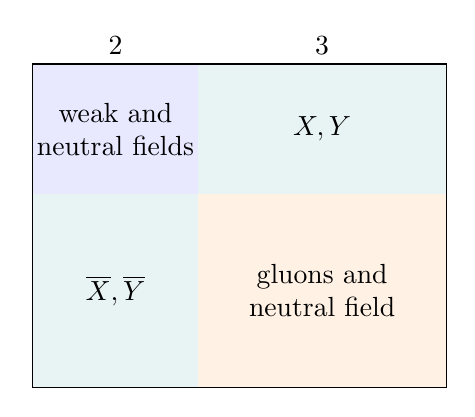
\begin{tikzpicture}[x=1.05cm,y=0.82cm]
  \draw[thick] (0,0) rectangle (5,5);
  \draw[thick] (2,0) -- (2,5);
  \draw[thick] (0,3) -- (5,3);
  \fill[blue!9] (0,3) rectangle (2,5);
  \fill[orange!10] (2,0) rectangle (5,3);
  \fill[teal!9] (2,3) rectangle (5,5);
  \fill[teal!9] (0,0) rectangle (2,3);
  \node[align=center] at (1,4) {weak and\\neutral fields};
  \node[align=center] at (3.5,1.5) {gluons and\\neutral field};
  \node[align=center] at (3.5,4) {\(X,Y\)};
  \node[align=center] at (1,1.5) {\(\overline X,\overline Y\)};
  \node[above] at (1,5) {\(2\)};
  \node[above] at (3.5,5) {\(3\)};
\end{tikzpicture}
\caption{La estructura en bloques \(2\oplus3\) del campo gauge de \(SU(5)\). Los bloques no diagonales conectan leptones y campos coloreados.}
\label{fig:l10-gauge-blocks}
\end{figure}

Con \(Q=T_3+Y\), el doblete débil coloreado de ~\eqref{eq:l10-adjoint-sm} tiene cargas \(-\tfrac13\) y \(-\tfrac43\); su conjugado tiene cargas \(+\tfrac13\) y \(+\tfrac43\). La lección llama \(X\) y \(Y\) a estas partículas, pero se abstiene explícitamente de asignar cada nombre a una carga determinada. La transición y la carga son el contenido invariante.

\begin{classroomqa}
\audiencequestion{¿Hay tres versiones de cada nuevo bosón gauge \(X\) o \(Y\)? \lecturetimestamp{00:41:28}}
\lecturerresponse{Sí. Una transición conecta una entrada de quark coloreada con una entrada leptónica sin color, por lo que el bosón intercambiado debe llevar el color que falta. Los campos \(X/Y\) forman tripletes de color y pueden emitir o absorber gluones.}
\end{classroomqa}

No se observan partículas coloreadas como estados asintóticos aislados. Los nuevos bosones gauge deben desintegrarse o hadronizarse en combinaciones neutras de color, igual que los quarks.

\section{Por qué el multiplete contiene antiquarks down}

Los generadores de \(SU(N)\) son matrices hermíticas sin traza. Para ver la relación con la palabra «especial», escribamos un elemento infinitesimal del grupo como
\begin{equation}
U(\epsilon)=e^{i\epsilon T}.
\end{equation}
La unitariedad da \(T^\dagger=T\), mientras que
\begin{equation}
1=\det U=e^{i\epsilon\operatorname{tr}T}
\end{equation}
para \(\epsilon\) arbitrario da
\begin{equation}
\operatorname{tr}T=0.
\label{eq:l10-traceless-generator}
\end{equation}

La carga eléctrica es una combinación lineal de generadores. Sobre la columna de materia de ~\eqref{eq:l10-fivebar}, actúa como
\begin{equation}
Q_{\overline5}
=
\operatorname{diag}
\left(0,-1,\frac13,\frac13,\frac13\right),
\qquad
\operatorname{tr}Q_{\overline5}=0.
\label{eq:l10-charge-fivebar}
\end{equation}
Por tanto,
\begin{equation}
0-1+3\left(\frac13\right)=0.
\end{equation}
Si se reemplazaran los campos de antiquark down por campos de quark down, se obtendría, en cambio,
\begin{equation}
0-1+3\left(-\frac13\right)=-2,
\end{equation}
que no puede ser la traza de un generador de \(SU(5)\). Así, la aparentemente extraña asignación de antiquarks down viene impuesta por la estructura del grupo.

\section{Los diez fermiones restantes}

Los otros diez campos surgen de un tensor antisimétrico de dos índices. En la convención estándar, este es la parte antisimétrica de
\begin{equation}
\mathbf5\otimes\mathbf5
=\mathbf{15}_S\oplus\mathbf{10}_A.
\label{eq:l10-five-five}
\end{equation}
La lección lo construye escribiendo temporalmente los números cuánticos conjugados
\begin{equation}
\chi=
\begin{pmatrix}
\nu^c\\
e^c\\
d_r\\
d_g\\
d_b
\end{pmatrix}.
\label{eq:l10-aux-five}
\end{equation}
Se trata de un recurso contable para formar productos tensoriales de representaciones, no de afirmar que exista un segundo multiplete físico de cinco partículas compuestas.

Sea
\begin{equation}
\Psi^{ij}=-\Psi^{ji},
\qquad
i,j=1,\ldots,5.
\label{eq:l10-antisym-ten}
\end{equation}
Todas las entradas diagonales son nulas y las entradas del triángulo inferior quedan determinadas por las del triángulo superior. Por tanto,
\begin{equation}
\dim\mathbf{10}
=\binom52
=\frac{5\cdot4}{2}
=10.
\label{eq:l10-ten-count}
\end{equation}

La carga eléctrica de una entrada es la suma de las cargas de fila y columna en ~\eqref{eq:l10-aux-five}. De ahí se obtiene inmediatamente \(e^c\) en la posición débil--débil, los quarks down y up en los bloques débil--color, y los campos de anti-up en el bloque color--color.

\begin{classroomqa}
\audiencequestion{Al combinar las etiquetas del positrón y del quark down, ¿debería la entrada resultante ser un bosón \(X\)? \lecturetimestamp{00:53:08}}
\lecturerresponse{No. En esta etapa construimos la representación de los fermiones, no la representación adjunta de los bosones gauge. Las cargas se suman como \(1-\tfrac13=\tfrac23\), así que la entrada tiene los números cuánticos de un quark up.}
\end{classroomqa}

Una elección coherente de los signos de color es
\begin{equation}
\Psi^{ij}=
\begin{pmatrix}
0 & e^c & d_r & d_g & d_b\\
-e^c & 0 & u_r & u_g & u_b\\
-d_r & -u_r & 0 & u_b^c & -u_g^c\\
-d_g & -u_g & -u_b^c & 0 & u_r^c\\
-d_b & -u_b & u_g^c & -u_r^c & 0
\end{pmatrix}.
\label{eq:l10-ten-matrix}
\end{equation}
Cambiar las fases de los campos modifica algunos signos mostrados, pero no la representación ni el contenido de partículas.

\begin{figure}[htbp]
\centering
\includegraphics[width=0.83\textwidth]{lecture_10_figure_05.png}
\lectureframe{00:59:17.500}
\caption{La matriz antisimétrica de materia \(2\oplus3\), sin obstrucciones, una vez comprobadas en clase las entradas y las etiquetas de color.}
\label{fig:l10-ten-board}
\end{figure}

\begin{classroomqa}
\audiencequestion{¿Hay que escribir la representación de dimensión diez como una matriz o se puede escribir como una columna? \lecturetimestamp{00:56:24}}
\lecturerresponse{Se puede hacer de las dos maneras. Se pueden enumerar en una columna las diez componentes independientes, pero la matriz antisimétrica \(5\times5\) muestra cómo \(SU(5)\) actúa sobre sus dos índices y, por tanto, es mucho más informativa.}
\end{classroomqa}

\begin{classroomqa}
\audiencequestion{En el bloque color--color, ¿la entrada marcada \(u\) debería ser en realidad un campo de anti-up? \lecturetimestamp{00:57:51}}
\lecturerresponse{Sí. La etiqueta de la pizarra se corrige a \(u^c\), un campo de anti-up levógiro. La suma de las cargas de dos estados de la base de tipo down es \(-\tfrac23\), que es la carga eléctrica de un antiquark up.}
\end{classroomqa}

\begin{classroomqa}
\audiencequestion{Se omitieron los colores de varias entradas de la matriz. ¿Se conservan de todos modos? \lecturetimestamp{00:58:05}}
\lecturerresponse{Sí. Las tres posiciones de color son rojo, verde y azul. Las etiquetas se omitieron únicamente para reducir el desorden.}
\end{classroomqa}

Un par antisimétrico de fundamentales de color se transforma como un anticolor:
\begin{equation}
\wedge^2\mathbf3\simeq\overline{\mathbf3},
\qquad
(rg,rb,gb)\sim(\overline b,-\overline g,\overline r).
\label{eq:l10-anticolor}
\end{equation}
Por eso, las tres entradas independientes del bloque color--color forman precisamente el triplete de color de anti-up.

Ahora, una generación queda organizada como
\begin{equation}
\overline{\mathbf5}\oplus\mathbf{10}.
\label{eq:l10-family}
\end{equation}
Es notable que \(u_L\) y \(u^c_L\) aparezcan en un mismo multiplete irreducible, mientras que \(d_L\) y \(d^c_L\), o \(e_L\) y \(e^c_L\), pertenecen a multipletes distintos.

\begin{classroomqa}
\audiencequestion{Si las transformaciones gauge actúan solo dentro de cada representación, ¿cómo puede una masa conectar campos que pertenecen al cinco conjugado y al diez? \lecturetimestamp{01:00:40}}
\lecturerresponse{Los bosones gauge no transforman una representación irreducible de materia en la otra. Los campos de Higgs y los acoplamientos de Yukawa pueden conectar representaciones distintas y, a la vez, formar una interacción globalmente invariante bajo \(SU(5)\); cuando el campo de Higgs adquiere un valor esperado, esas interacciones generan masas.}
\end{classroomqa}

\section{Los bosones gauge actúan como desplazamientos}

Una vez ensamblada la representación, la acción de un bosón gauge se puede interpretar como un desplazamiento entre sus entradas. Un bosón neutro puede dejar una etiqueta sin cambios; un bosón débil desplaza entre posiciones débiles, un gluón entre posiciones de color y un bosón \(X/Y\) entre posiciones débiles y de color. Los bosones gauge cargados tienen antipartículas, por lo que cada desplazamiento cuenta con un proceso inverso.

En el caso del tensor antisimétrico, una transformación infinitesimal actúa sobre cualquiera de los dos índices:
\begin{equation}
\delta\Psi^{ij}
=
i\epsilon
\left(
T^i{}_k\Psi^{kj}
+
T^j{}_k\Psi^{ik}
\right).
\label{eq:l10-two-index-action}
\end{equation}
En la representación matricial, el primer término desplaza verticalmente y el segundo, horizontalmente. Las etiquetas de las partículas constituyentes usadas para construir el tensor son solo un recurso mnemotécnico; ~\eqref{eq:l10-two-index-action} es el enunciado exacto en términos de la teoría de grupos.

Los desplazamientos débiles transforman \(d\) en \(u\), el proceso a nivel de quarks que está detrás de la desintegración beta del neutrón. Los desplazamientos de color cambian rojo, verde y azul sin cambiar el sabor. Los desplazamientos no diagonales hacen algo nuevo:
\begin{equation}
\begin{aligned}
d^c&\longleftrightarrow e,
& d^c&\longleftrightarrow\nu,\\
d&\longleftrightarrow u^c,
& u&\longleftrightarrow e^c,
\end{aligned}
\label{eq:l10-leptoquark-shifts}
\end{equation}
con el campo \(X/Y\) apropiado llevando la diferencia de carga y de color.

\begin{classroomqa}
\audiencequestion{¿Qué representan los desplazamientos entre la cuarta y la quinta posición, y qué ocurre con un desplazamiento de la primera a la cuarta? \lecturetimestamp{01:10:36}}
\lecturerresponse{El desplazamiento de la cuarta--a la quinta cambia un color por otro y es una transición de gluón. El desplazamiento de la primera--a la cuarta cruza entre los bloques débil y de color y corresponde a una de las nuevas transiciones \(X/Y\).}
\end{classroomqa}

\begin{classroomqa}
\audiencequestion{¿Se puede rellenar explícitamente una entrada de la mitad inferior de la matriz antisimétrica? \lecturetimestamp{01:11:23}}
\lecturerresponse{Sí. Cada entrada del triángulo inferior es el negativo de la entrada transpuesta correspondiente del triángulo superior. Rellenar una hace visible la regla; rellenarlas todas no añade estados nuevos.}
\end{classroomqa}

\section{La peligrosa consecuencia: la desintegración del protón}

Un bosón \(X/Y\) puede acoplar un quark a un leptón en un vértice y dos campos de tipo quark en otro. Para momentos mucho menores que su masa, integrar el bosón pesado da una interacción de dimensión seis, de la forma esquemática
\begin{equation}
\mathcal L_{\mathrm{eff}}
\sim
\frac{g_5^2}{M_X^2}\,(qq)(q\ell)
+\text{h.c.}
\label{eq:l10-effective-proton}
\end{equation}
Esta interacción viola por separado los números bariónico y leptónico, a la vez que conserva las combinaciones que impone la interacción gauge unificada.

La pizarra sigue un quark down y un quark up a través del intercambio pesado. El quark down se convierte en un positrón, el quark up en un antiquark up y un segundo quark up actúa de espectador:
\begin{equation}
uud
\longrightarrow
e^++u\overline u.
\label{eq:l10-quark-decay}
\end{equation}
El estado inicial es un protón. El par \(u\overline u\) puede hadronizarse en un pión neutro, dando
\begin{equation}
p\longrightarrow e^++\pi^0.
\label{eq:l10-proton-pion}
\end{equation}

\begin{figure}[htbp]
\centering
\includegraphics[width=0.82\textwidth]{lecture_10_figure_06.png}
\lectureframe{01:16:02.500}
\caption{Construcción completa en la pizarra del intercambio de un bosón pesado dentro de un protón, donde se ven el quark up espectador y el canal del positrón.}
\label{fig:l10-proton-board}
\end{figure}

La lección también menciona \(p\to e^++\gamma\), en el que el par quark--antiquark se aniquila electromagnéticamente. Ese canal sufre una supresión electromagnética adicional respecto de la hadronización directa.

Esta posibilidad no es un adorno opcional del modelo. Cuando un grupo simple contiene generadores que conectan quarks y leptones, en general se esperan procesos que violan el número bariónico. Si ocurrieran en escalas de tiempo débiles o electromagnéticas ordinarias, no sobrevivirían los núcleos, el hidrógeno ni la materia macroscópica.

\section{¿Por qué el protón tiene una vida tan larga?}

\begin{classroomqa}
\audiencequestion{¿El acoplamiento que produce un bosón \(X\) es el mismo acoplamiento unificado que usa el resto del grupo? \lecturetimestamp{01:18:34}}
\lecturerresponse{Sí, a la escala de unificación. Una teoría gauge simple de \(SU(5)\) tiene un solo acoplamiento gauge \(g_5\). Los acoplamientos fuerte, débil y de hipercarga a baja energía difieren porque evolucionan de maneras distintas después de la ruptura de la simetría unificada.}
\end{classroomqa}

No se puede elegir un acoplamiento desmesuradamente pequeño sin abandonar la estructura unificada. La supresión disponible proviene del propagador pesado:
\begin{equation}
\mathcal A
\sim
\frac{g_5^2}{M_X^2}.
\label{eq:l10-amplitude}
\end{equation}
Al elevar al cuadrado la amplitud aparece \(g_5^4/M_X^4\). El análisis dimensional y el elemento de matriz del protón completan la estimación de la tasa de desintegración:
\begin{equation}
\Gamma_p
\sim
C_{\mathrm{had}}\,
\frac{\alpha_5^2\,m_p^5}{M_X^4},
\qquad
\alpha_5=\frac{g_5^2}{4\pi},
\label{eq:l10-rate}
\end{equation}
donde \(C_{\mathrm{had}}\) contiene factores de grupo, efectos de renormalización y el elemento de matriz hadrónico no perturbativo.

\editorialnote{La lección destaca la dependencia esencial en \(g^4/M_X^4\) y señala que se omiten los factores de masa del protón. La ecuación~\eqref{eq:l10-rate} restituye la dimensión de masa necesaria, sin pretender ofrecer un cálculo preciso de la vida media.}

\begin{classroomqa}
\audiencequestion{¿El pequeño factor \(g^4\), quizá del orden de \(10^{-8}\) según la estimación aproximada hecha en clase, basta ya para que la vida media sea lo bastante larga? \lecturetimestamp{01:25:13}}
\lecturerresponse{No. Ayuda, pero la diferencia entre un tiempo microscópico de interacción fuerte y el límite de vida media del protón abarca muchos más órdenes de magnitud. La cuarta potencia de la masa pesada debe proporcionar la supresión decisiva.}
\end{classroomqa}

Si todas las masas fueran del orden de la masa del protón, la unidad natural de tiempo sería aproximadamente el tiempo que tarda la luz en atravesar un protón:
\begin{equation}
t_p\sim\frac{1\ \mathrm{fm}}{c}\sim10^{-23}\ \mathrm{s}.
\label{eq:l10-proton-time}
\end{equation}
La mera existencia de protones primordiales ya muestra que su vida media supera la edad del universo, pero las búsquedas de laboratorio van muchísimo más lejos. La lección compara la estimación microscópica con el límite experimental citado entonces
\begin{equation}
\tau_p\gtrsim10^{33}\ \mathrm{yr}.
\label{eq:l10-lifetime-bound}
\end{equation}

No hace falta observar un solo protón durante tanto tiempo. Si la vida media fuera de \(10^{15}\) años, una muestra de \(10^{15}\) protones produciría aproximadamente un evento al año. En general, para \(N_p\) protones observados durante un tiempo \(T\), el número esperado de desintegraciones es
\begin{equation}
\langle n\rangle\simeq\frac{N_pT}{\tau_p}.
\label{eq:l10-event-count}
\end{equation}
Un detector con aproximadamente \(10^{33}\) protones es un tanque grande, no un objeto astronómico: los protones en sí tienen una masa del orden de \(10^6\) kilogramos. Observar una muestra así convierte una vida media individual enorme en una tasa de eventos medible o en un límite inferior más estricto.

Al combinar ~\eqref{eq:l10-rate} con la restricción sobre la vida media, la masa del bosón gauge leptoquark debe acercarse a
\begin{equation}
M_X\sim10^{15}\text{--}10^{16}\ \mathrm{GeV},
\label{eq:l10-mx}
\end{equation}
La lección utiliza \(10^{16}\,\mathrm{GeV}\) como la escala segura fácil de recordar. Está varios órdenes de magnitud por debajo de la escala de Planck y, por tanto, no es automáticamente incompatible con la teoría cuántica de campos.

\section{Ruptura de \texorpdfstring{\(SU(5)\)}{SU(5)} y escala de unificación}

Los campos \(X/Y\) comparten un multiplete adjunto de \(SU(5)\) con los campos gauge del Modelo Estándar. Una simetría gauge exacta y no rota no permitiría que algunos de sus miembros tuvieran masas cercanas a \(10^{16}\,\mathrm{GeV}\) mientras el fotón y los gluones permanecen sin masa. Por tanto, la simetría debe romperse espontáneamente.

\begin{classroomqa}
\audiencequestion{Si la simetría \(SU(5)\) no se rompiera, ¿serían sin masa todos sus bosones gauge? \lecturetimestamp{01:29:37}}
\lecturerresponse{Sí, en la teoría gauge que estamos considerando. La invariancia gauge prohíbe una masa común explícita. El mecanismo de Higgs puede dar masa a los bosones gauge asociados a generadores rotos y dejar sin masa los campos gauge del subgrupo no roto.}
\end{classroomqa}

El mecanismo de Higgs electrodébil ya ilustra este patrón: distingue el fotón de \(W^\pm\) y \(Z\). La gran unificación requiere un parámetro de orden independiente a alta escala, que distinga el bloque débil \(2\) del bloque de color \(3\) y haga extremadamente pesados los campos no diagonales \(X/Y\).

En comparación con \(10^{16}\,\mathrm{GeV}\), incluso una masa de bosón débil de \(100\,\mathrm{GeV}\) es despreciable. Muy por encima del umbral de masa pesada, se pueden despreciar todas las masas de los bosones gauge y la simetría completa \(SU(5)\) pasa a ser una buena aproximación. Esto es lo que significa una escala de unificación: no que el mundo de baja energía tenga manifiestamente \(SU(5)\), sino que los procesos a energías suficientemente altas se vuelven insensibles a las diferencias de masa debidas a la ruptura de simetría.

\section{Acoplamientos variables con la escala}

Los acoplamientos gauge dependen logarítmicamente de la escala de energía. Si definimos
\begin{equation}
\alpha_i(\mu)=\frac{g_i^2(\mu)}{4\pi},
\end{equation}
la evolución a un bucle tiene la forma
\begin{equation}
\alpha_i^{-1}(\mu)
=
\alpha_i^{-1}(\mu_0)
-\frac{b_i}{2\pi}
\ln\!\left(\frac{\mu}{\mu_0}\right).
\label{eq:l10-running}
\end{equation}
Los coeficientes \(b_i\) dependen del grupo gauge y de todas las partículas lo bastante ligeras como para circular en los bucles cuánticos pertinentes.

\editorialnote{Para comparar la hipercarga con los acoplamientos no abelianos dentro de \(SU(5)\), hay que dar a \(g_1\) la normalización convencional de gran unificación. Este es el origen de los factores numéricos de teoría de grupos mencionados en la lección.}

A energías de laboratorio, los inversos de los tres acoplamientos son distintos. Según el orden cualitativo expuesto en la clase, \(1/\alpha_1\) es el mayor porque la hipercarga es la interacción más débil; le sigue \(1/\alpha_2\), y \(1/\alpha_3\) es el menor porque la interacción fuerte es la más intensa. Las curvas a energías inaccesibles no se miden directamente. Se calculan a partir de los valores observados a baja energía, del espectro de partículas y de los diagramas de bucles que determinan las funciones beta. Con el contenido de partículas del Modelo Estándar, se vuelven casi rectas al representarlas frente a \(\log\mu\).

\begin{figure}[htbp]
\centering
\includegraphics[width=0.74\textwidth]{lecture_10_figure_07.png}
\lectureframe{01:36:32.500}
\caption{Gráfica dibujada en la pizarra que muestra cómo los acoplamientos de gauge inversos se aproximan entre sí cerca de \(10^{16}\,\mathrm{GeV}\). La región rodeada con un círculo señala que no llegan a coincidir exactamente.}
\label{fig:l10-running-board}
\end{figure}

Por debajo de la escala de unificación, la simetría está rota, el espectro ligero no completa multipletes degenerados de \(SU(5)\) y los tres coeficientes de las funciones beta son distintos. Por consiguiente, los acoplamientos evolucionan a ritmos diferentes. A la escala alta, cabe preguntarse si alcanzan un valor común:
\begin{equation}
\alpha_1(M_{\mathrm{GUT}})
\stackrel{?}{=}
\alpha_2(M_{\mathrm{GUT}})
\stackrel{?}{=}
\alpha_3(M_{\mathrm{GUT}}).
\label{eq:l10-unification-condition}
\end{equation}

Con solo el espectro del Modelo Estándar no supersimétrico, las líneas se aproximan entre sí en torno a \(10^{15}\)--\(10^{16}\,\mathrm{GeV}\), pero no llegan a coincidir: la discrepancia es apreciable; en la clase, el acuerdo se describe como de aproximadamente un quince por ciento. La coincidencia importante es que esta es también la escala que exige la estabilidad del protón.

\section{Una última pregunta sobre el neutrón}

\begin{classroomqa}
\audiencequestion{Si en el diagrama de desintegración del protón se sustituyera el quark up espectador por un quark down, ¿describiría esto la desintegración del neutrón? ¿Sería relevante el bosón \(X\)? \lecturetimestamp{01:36:40}}
\lecturerresponse{Definiría un canal de desintegración del neutrón propio de una teoría de gran unificación, como \(n\to e^++\pi^-\), pero no sería la desintegración conocida de un neutrón libre. La desintegración beta ordinaria del neutrón es \(n\to p+e^-+\overline\nu_e\) y ocurre mediante la interacción débil. Si se invirtiera el orden de masas entre el protón-- y el neutrón, también se invertiría la estabilidad frente a la desintegración beta, mientras que el canal de gran unificación, mucho más lento, podría seguir existiendo.}
\end{classroomqa}

Esta distinción separa la cinemática de la nueva interacción. Cuál de los dos nucleones se desintegra beta depende de la diferencia de masas entre el protón-- y el neutrón; la violación del número bariónico por intercambio de \(X/Y\) es un mecanismo independiente y enormemente suprimido.

\section{La supersimetría y una perspectiva más amplia}

La incorporación de un espectro de partículas supercompañeras modifica los coeficientes de las funciones beta en la ecuación~\eqref{eq:l10-running}. Según la explicación de la clase, entonces los tres acoplamientos extrapolados coinciden con una precisión de aproximadamente un uno por ciento. Esto no demuestra la supersimetría ni la gran unificación, pero sí explica por qué ambas ideas suelen tratarse conjuntamente.

Los multipletes de materia pueden unificarse aún más. Según
\begin{equation}
SO(10)\supset SU(5),
\end{equation}
una representación espinorial se descompone como
\begin{equation}
\mathbf{16}
\longrightarrow
\mathbf{10}\oplus\overline{\mathbf5}\oplus\mathbf1.
\label{eq:l10-so10}
\end{equation}
El singlete se identifica de forma natural con un antineutrino de quiralidad izquierda o, de manera equivalente, con el conjugado de carga de un neutrino de quiralidad derecha. Así, los dieciséis campos de una familia extendida caben en un único multiplete irreducible de \(SO(10)\).

Los experimentos de desintegración del protón siguen poniendo a prueba la idea: cuando no se observa ningún suceso, se eleva el límite inferior de su vida media. Los modelos supersimétricos de gran unificación no predicen una vida media única para el protón: los campos pesados adicionales y los operadores cuya forma depende de las partículas supercompañeras pueden modificar el canal dominante y la tasa en un amplio intervalo.

\editorialnote{En la gran unificación supersimétrica, el intercambio de Higgs con triplete de color puede generar operadores de dimensión cinco que violan el número bariónico, además del operador de dimensión seis mediado por bosones de gauge que se analiza aquí. Sus coeficientes dependen mucho del espectro pesado, de la estructura de sabores y de las masas de las partículas supercompañeras; esto explica la advertencia de la clase de que la supersimetría por sí sola no determina una vida media única.}

La lección que perdura es una tensión, no un veredicto. La teoría de grupos reúne quarks y leptones con una economía notable, la evolución de los acoplamientos apunta a una escala alta común y la supersimetría afina esa indicación numérica. Esta misma construcción también predice la peligrosa conversión de quarks en leptones. Por tanto, cualquier versión satisfactoria debe conservar la elegancia y, a la vez, mantener estable el protón durante un tiempo casi inconcebiblemente largo. Con el espíritu de las palabras finales de la clase: ojalá todos nuestros protones permanezcan estables.
